\section{Experimental Evaluation}
\label{sec:evaluation}

In this section we present the results from our extensive experiments again 
the audio captcha services presented in Section~\ref{sec:services}.

\begin{table*}[t]
\centering
\caption{Accuracy of different speech recognition services and accents against the audio captcha services we evaluated.}
\begin{tabular}{lccccc}
\toprule
&\multicolumn{5}{c}{\textbf{Speech Recognition Service (Accent)}}\\
\cmidrule{2-6}
\textbf{Captcha Service}& \textbf{Wit}& \textbf{IBM (US)} & \textbf{ IBM (UK)} & \textbf{Google (US)} & \textbf{Google (UK)} \\
\hline
Recaptcha v2.a & 67.1\% (671/1000) & 95.8\% (958/1000) & 67.2\% (672/1000) & \textbf{98.3\%} (983/1000) & 81.6\% (816/1000) \\
\rowcolor{Gray}
Recaptcha v2.b &  &  &  &  & \\
Apple  & 0\% (0/365)  & 2.3\% (6/260) & 6.8\% (17/251) & 35.8\% (126/352) & \textbf{52.8\%} (143/271) \\
\rowcolor{Gray}
BotDetect  & 1.23\% (11/894)  & 1.38\% (19/138) & 6.67\% (12/180) & \textbf{9.5\%} (102/1067)  & 6.65\% (79/1187) \\
Captchas.net  & 0\% (0/1008) & 1.1\% (9/778)  & 0.3\% (3/1010)  & 2.7\% (16/593) & \textbf{22.3\%} (230/1030) \\
\rowcolor{Gray}
Microsoft Live & &  &  & & \\
SecurImage  & 0\% (0/1000)  & 0\% (0/1000) & 0\% (0/1000) & 0.1\% (0/1000) & \textbf{3\%} (30/1000) \\
\rowcolor{Gray}
Telerik  & 21.2\% (142/668)  & \textbf{97\%} (452/466) & 12.9\% (47/364) & 74.2\% (150/202) & 49.3\% (112/217) \\
\bottomrule
\end{tabular}
\label{tab:combinations}
\end{table*}

\textbf{Attack accuracy.} Table~\ref{tab:combinations} presents the accuracy obtained by each speech recognition service 
against the audio captcha services. In cases where the speech recognition service has the option to select an accent,
we experiment with both American and British English. Surprisingly, we find that for every single captcha scheme, at least
one of the speech recognition services is able to solve more challenges than the 1\% threshold, thus, \emph{practically 
rendering all captcha schemes broken.} Nonetheless, there is significant variance, not only across captcha schemes, but
the accuracy obtained by each speech recognition engine for a specific captcha service. 

The most alarming finding is 
that \system achieved the highest accuracy against \re v2.a, the most widely deployed captcha service. When compared 
to the 70.78\% attack accuracy reported for the image \re~\cite{sivakorn:eurosp16}, it becomes apparent that audio challenges
weaken the overall security offered by \re, as fraudsters can target audio captchas for deploying highly successful
attacks. The Apple and Microsoft Live captchas that protect their account creation process, are also highly susceptible to 
automated attacks, as our approach correctly solves up to 52.8\% and X\% respectively.

While the presence of noise impacts the accuracy of the transcription process for all the respective captcha schemes
(see Table~\ref{tab:services}), none of the services is completely impervious to our attacks. Nonetheless, we
found that the audio captchas from Securimage are the most robust due to the presence of background semantic noise,
as \system was only able to solve 3\% of the challenges when using Google's Speech API and the British English accent
configuration. Another interesting observation was that no single speech recognition system or configuration that 
was consistently more accurate across all captchas; however, Google's speech recognition achieved the best
results for \note{X} out of the \note{Y} captcha schemes. While attackers could increase the attacks' accuracy
by first pre-processing the audio challenges so as to reduce the noise, the motivation behind our study is to 
demonstrate how attackers can employ off-the-shelf systems for breaking existing captcha systems.

\note{Rate limit of speech recognition services.}
\textbf{Solution flexibility.} \note{How many wrong digits allowed per service?}

\begin{figure*}[tp]
\begin{subfigure}{0.75\textwidth}
    \centering
    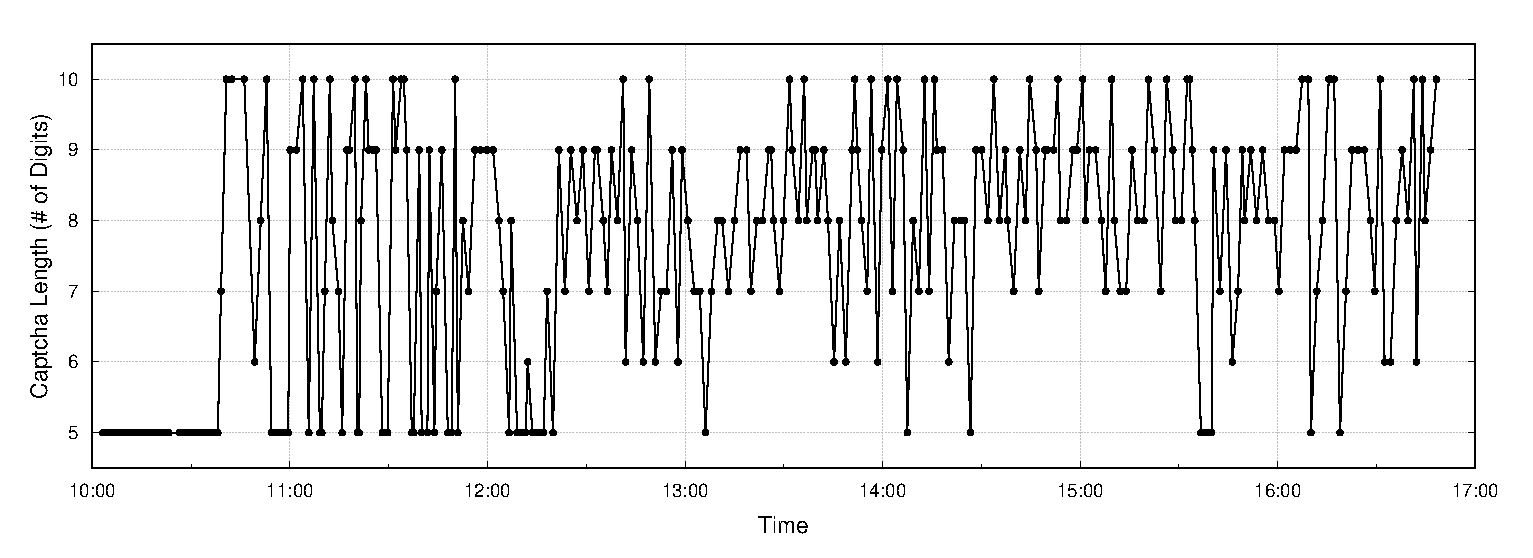
\includegraphics[width=1\textwidth]{figures/captcha_length.eps}
    \label{fig:length_time}
\end{subfigure} %\hspace{0.03\textwidth}
\begin{subfigure}{0.2\textwidth}
    \centering
    %\caption{Average solution time for each recognition service and accent against the audio captcha services we evaluated.}
    \label{tab:length}
    \begin{tabular}{lc}
    \toprule
    \textbf{Digits} & \textbf{\# of Captchas} \\
    \hline
    5 & 95 (31.3\%) \\
    \rowcolor{Gray} 
    6 & 14 (4.6\%) \\
    7 & 34 (11.2\%) \\
    \rowcolor{Gray} 
    8 & 51 (16.8\%) \\
    9 & 68 (22.4\%) \\
    \rowcolor{Gray} 
    10 & 41 (13.5\%)\\
    \bottomrule
    \end{tabular}
\end{subfigure}
\caption{Variation of audio captcha length in \re v2.a over time.}
\label{fig:length}
\end{figure*}

\textbf{\re adaptive length}.
While by default the length of \re v2.a was 5 digits, we found %that after multiple captcha solutions by our system,
that \re would adapt to the large amount of requests issued from our system and return captchas with more digits. 
In Figure~\ref{fig:length} we present a representative experiment that depicts the number of digits in the captchas
processed by our system over the course of 7 hours. The first 49 captchas all contained 5 digits, whereas the length
changed in a seemingly random fashion. As can be seen by the breakdown statistics in the Figure, apart from the default
version with 5 digits, the most common variation we came across contained 9 digits.
%Overall, out of the 303 challenged processed in the experiment, 95 (31.3\%)
%had a length of 5, 14 (4.6\%) had 6 digits, 34 (11.2\%) had 7, 51 (16.8\%) had 8 digits, 68 (22.4\%) had 9, and 41 
%(13.5\%) had 10 digits.

\begin{table}[t]
\centering
\caption{Average solution time for each recognition service and accent against the audio captcha services we evaluated.}
\begin{tabular}{lccccc}
\toprule
&\multicolumn{5}{c}{\textbf{Speech Recognition Service}}\\
\cmidrule{2-6}
& & \textbf{(US)} & \textbf{(UK)} & \textbf{(US)} & \textbf{(UK)} \\
\textbf{Captcha}&  \textbf{Wit} & \textbf{IBM} & \textbf{IBM} & \textbf{Google} & \textbf{Google} \\
\hline
Recaptcha v2.a & 13.85s & 10.56s  & 12.25s & \textbf{18.46s} & 20.41s \\
\rowcolor{Gray}
Recaptcha v2.b &  &  &  & & \\
Apple  & 36.4s & 33.4s  & 34.7s & 15.5s & \textbf{13.9s} \\
\rowcolor{Gray}
BotDetect  & 5.53s  & 4.21s & 5.72s & \textbf{3.40s} & 3.05s \\
Captchas.net  & 19.92s  & 14.62s  & 15.65s  & 7.56s & \textbf{7.79s} \\
\rowcolor{Gray}
Microsoft Live & &  &  & & \\
SecurImage  & 34.31s & 23.60s & 25.10s  & 27.29s & \textbf{35.28s} \\
\rowcolor{Gray}
Telerik  & & & & & \\
\bottomrule
\end{tabular}
\label{tab:solution_time}
\end{table}

\textbf{Solution time.} In Table~\ref{tab:solution_time} we include the average time required by each speech recognition 
service for returning a transcription of the audio captcha. The bold values denote the combination that achieved the highest 
accuracy for that captcha scheme.

\note{How many mistakes allowed for a correct answer?}

\textbf{Economic analysis.}
\note{Length of challenge, cost per minute for solver. reselling solved tokens. How much profit?}
IBM Watson: It is available for free for the first 1000 min/per month for each account, after which each additional minute is charged \$0.02.
